\documentclass[aspectratio=169]{beamer}

% 引入中文支持
\usepackage{ctex}
% 引入插图宏包
\usepackage{graphicx}

% 选择一个简洁的主题（可选，这里使用默认的清爽样式）
\usetheme{default}
% 去除右下角的 PDF 导航符号，让页面更整洁
\setbeamertemplate{navigation symbols}{}

\begin{document}

% 第一页
\begin{frame}{用户关怀 —— 无障碍设施信息展示与筛选}
    \centering
    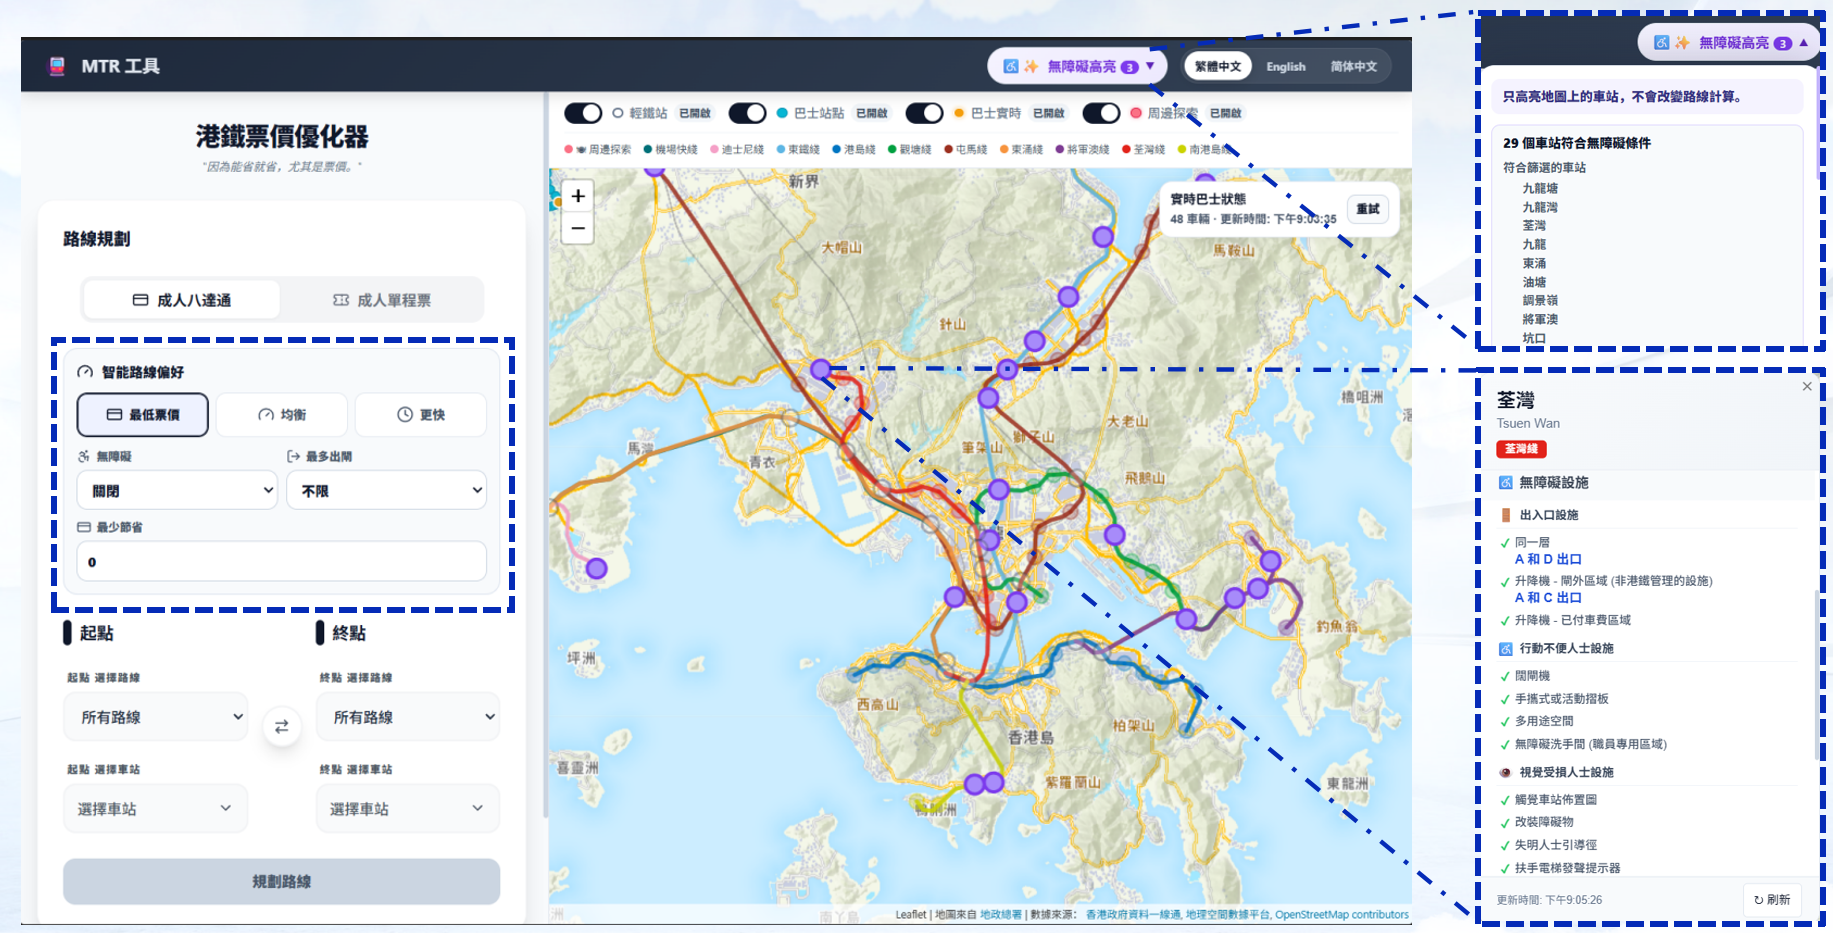
\includegraphics[width=0.95\textwidth,height=0.8\textheight,keepaspectratio]{Part 4-Page 1.png}
\end{frame}

% 第二页
\begin{frame}{用户关怀 —— 让票价优化更贴近真实出行决策}
    \centering
    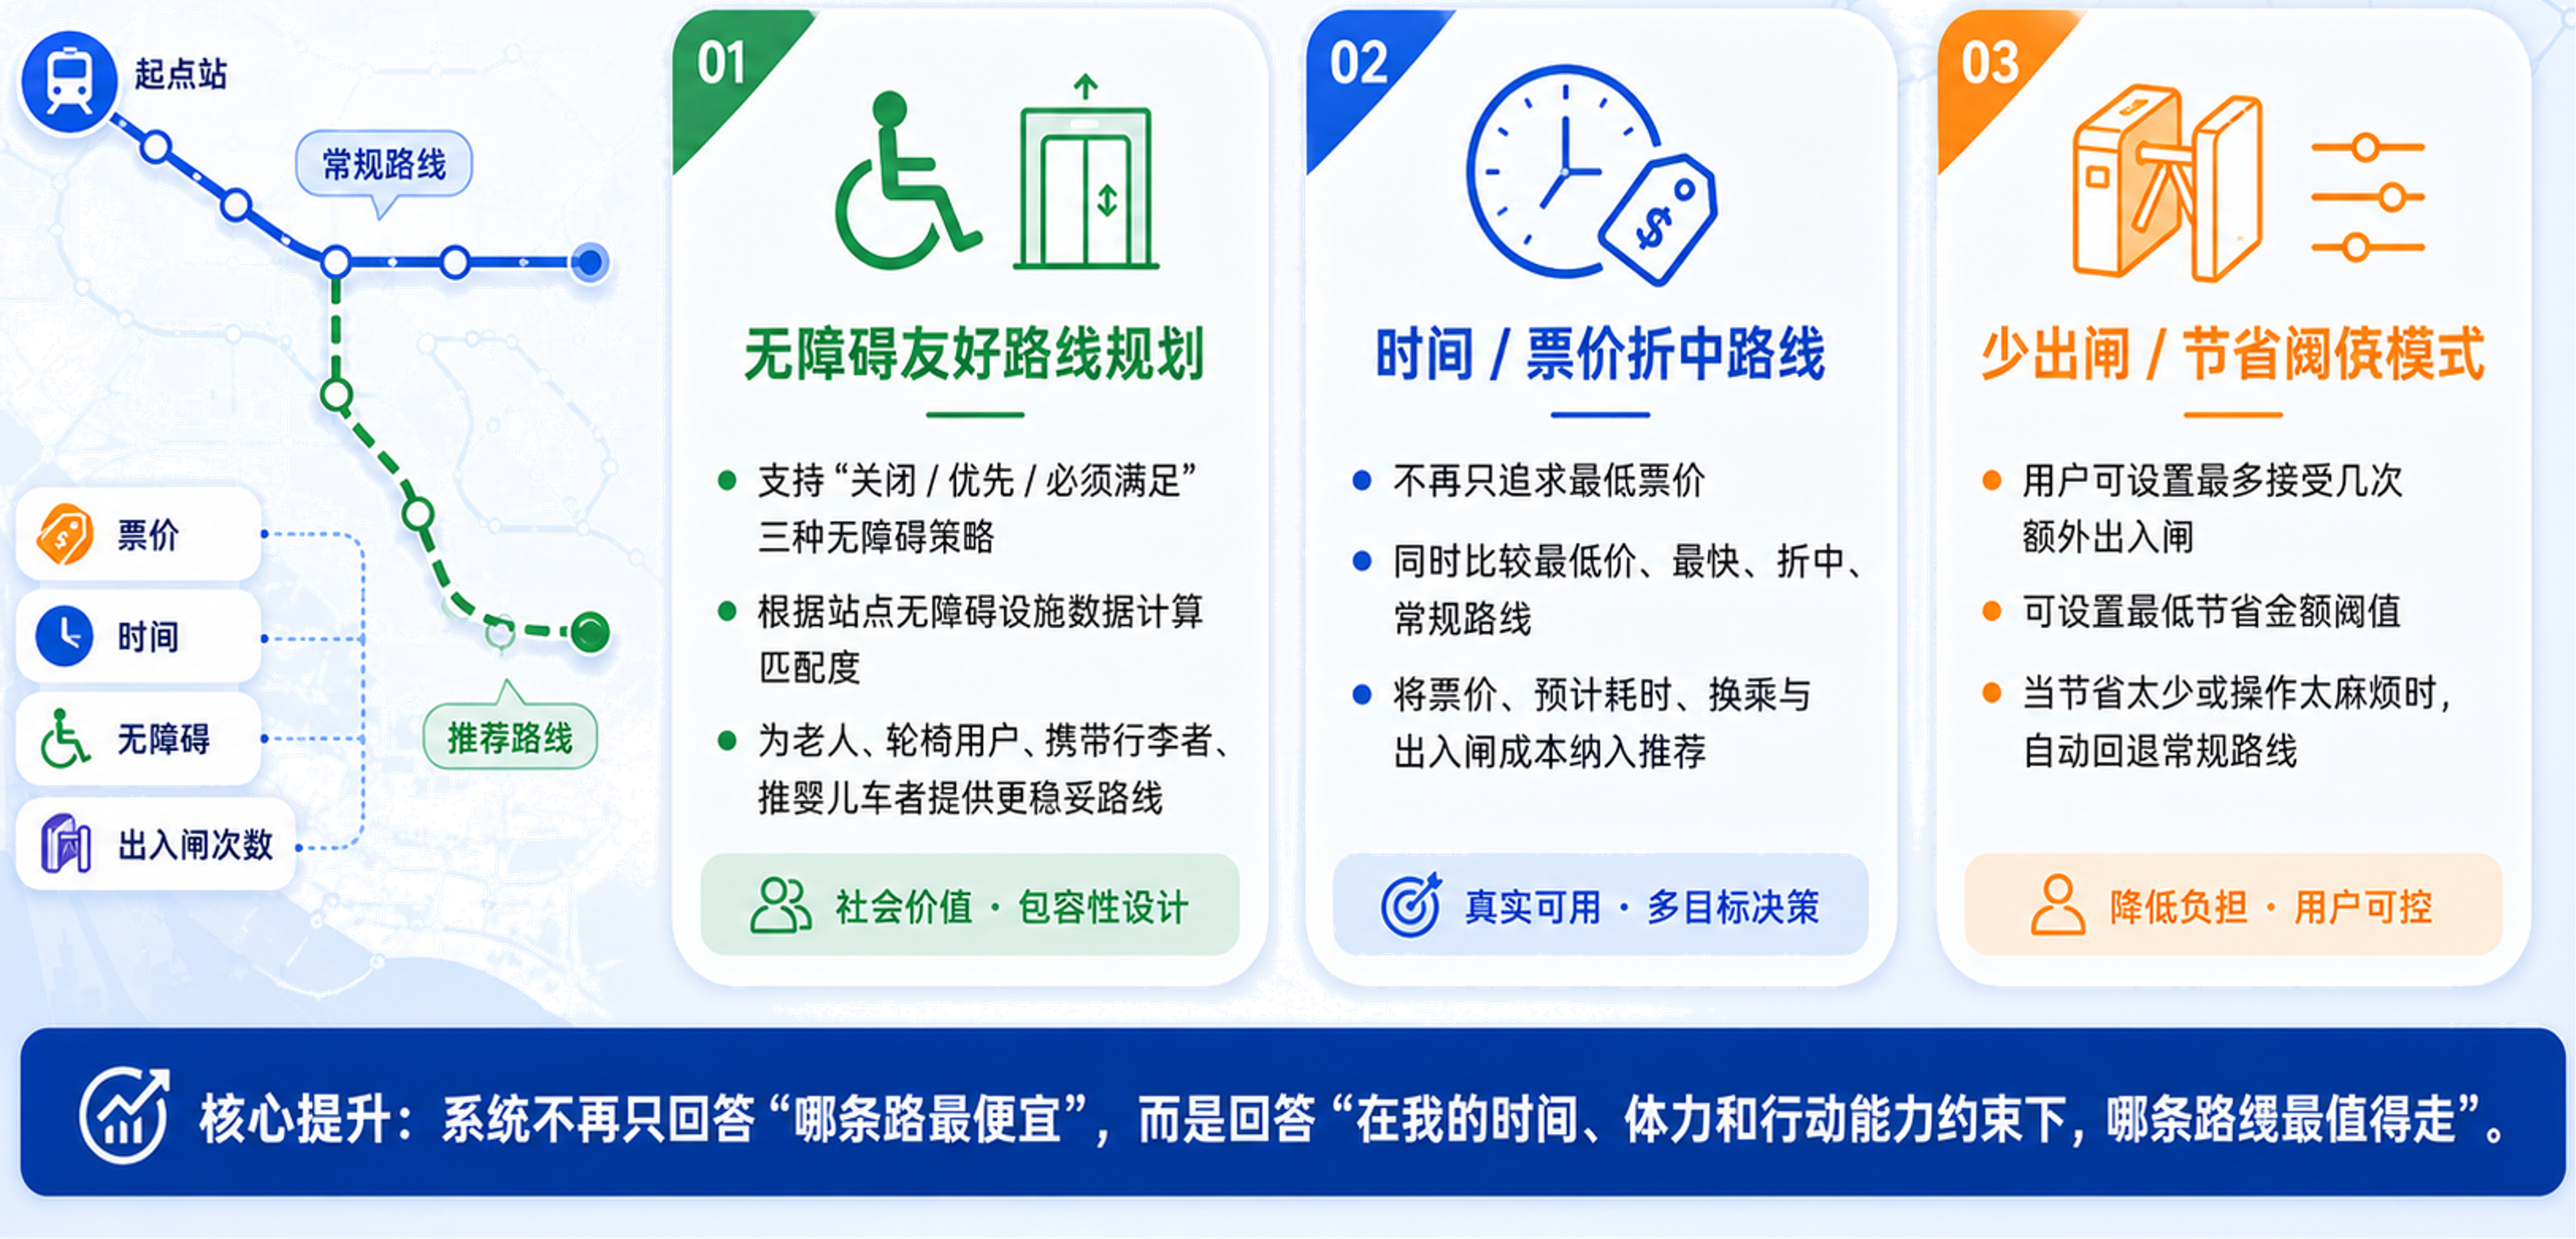
\includegraphics[width=0.95\textwidth,height=0.8\textheight,keepaspectratio]{Part 4-Page 2.png}
\end{frame}

% 第三页
\begin{frame}{用户关怀 —— 把“用户偏好”转化为“可解释的路线推荐”}
    \centering
    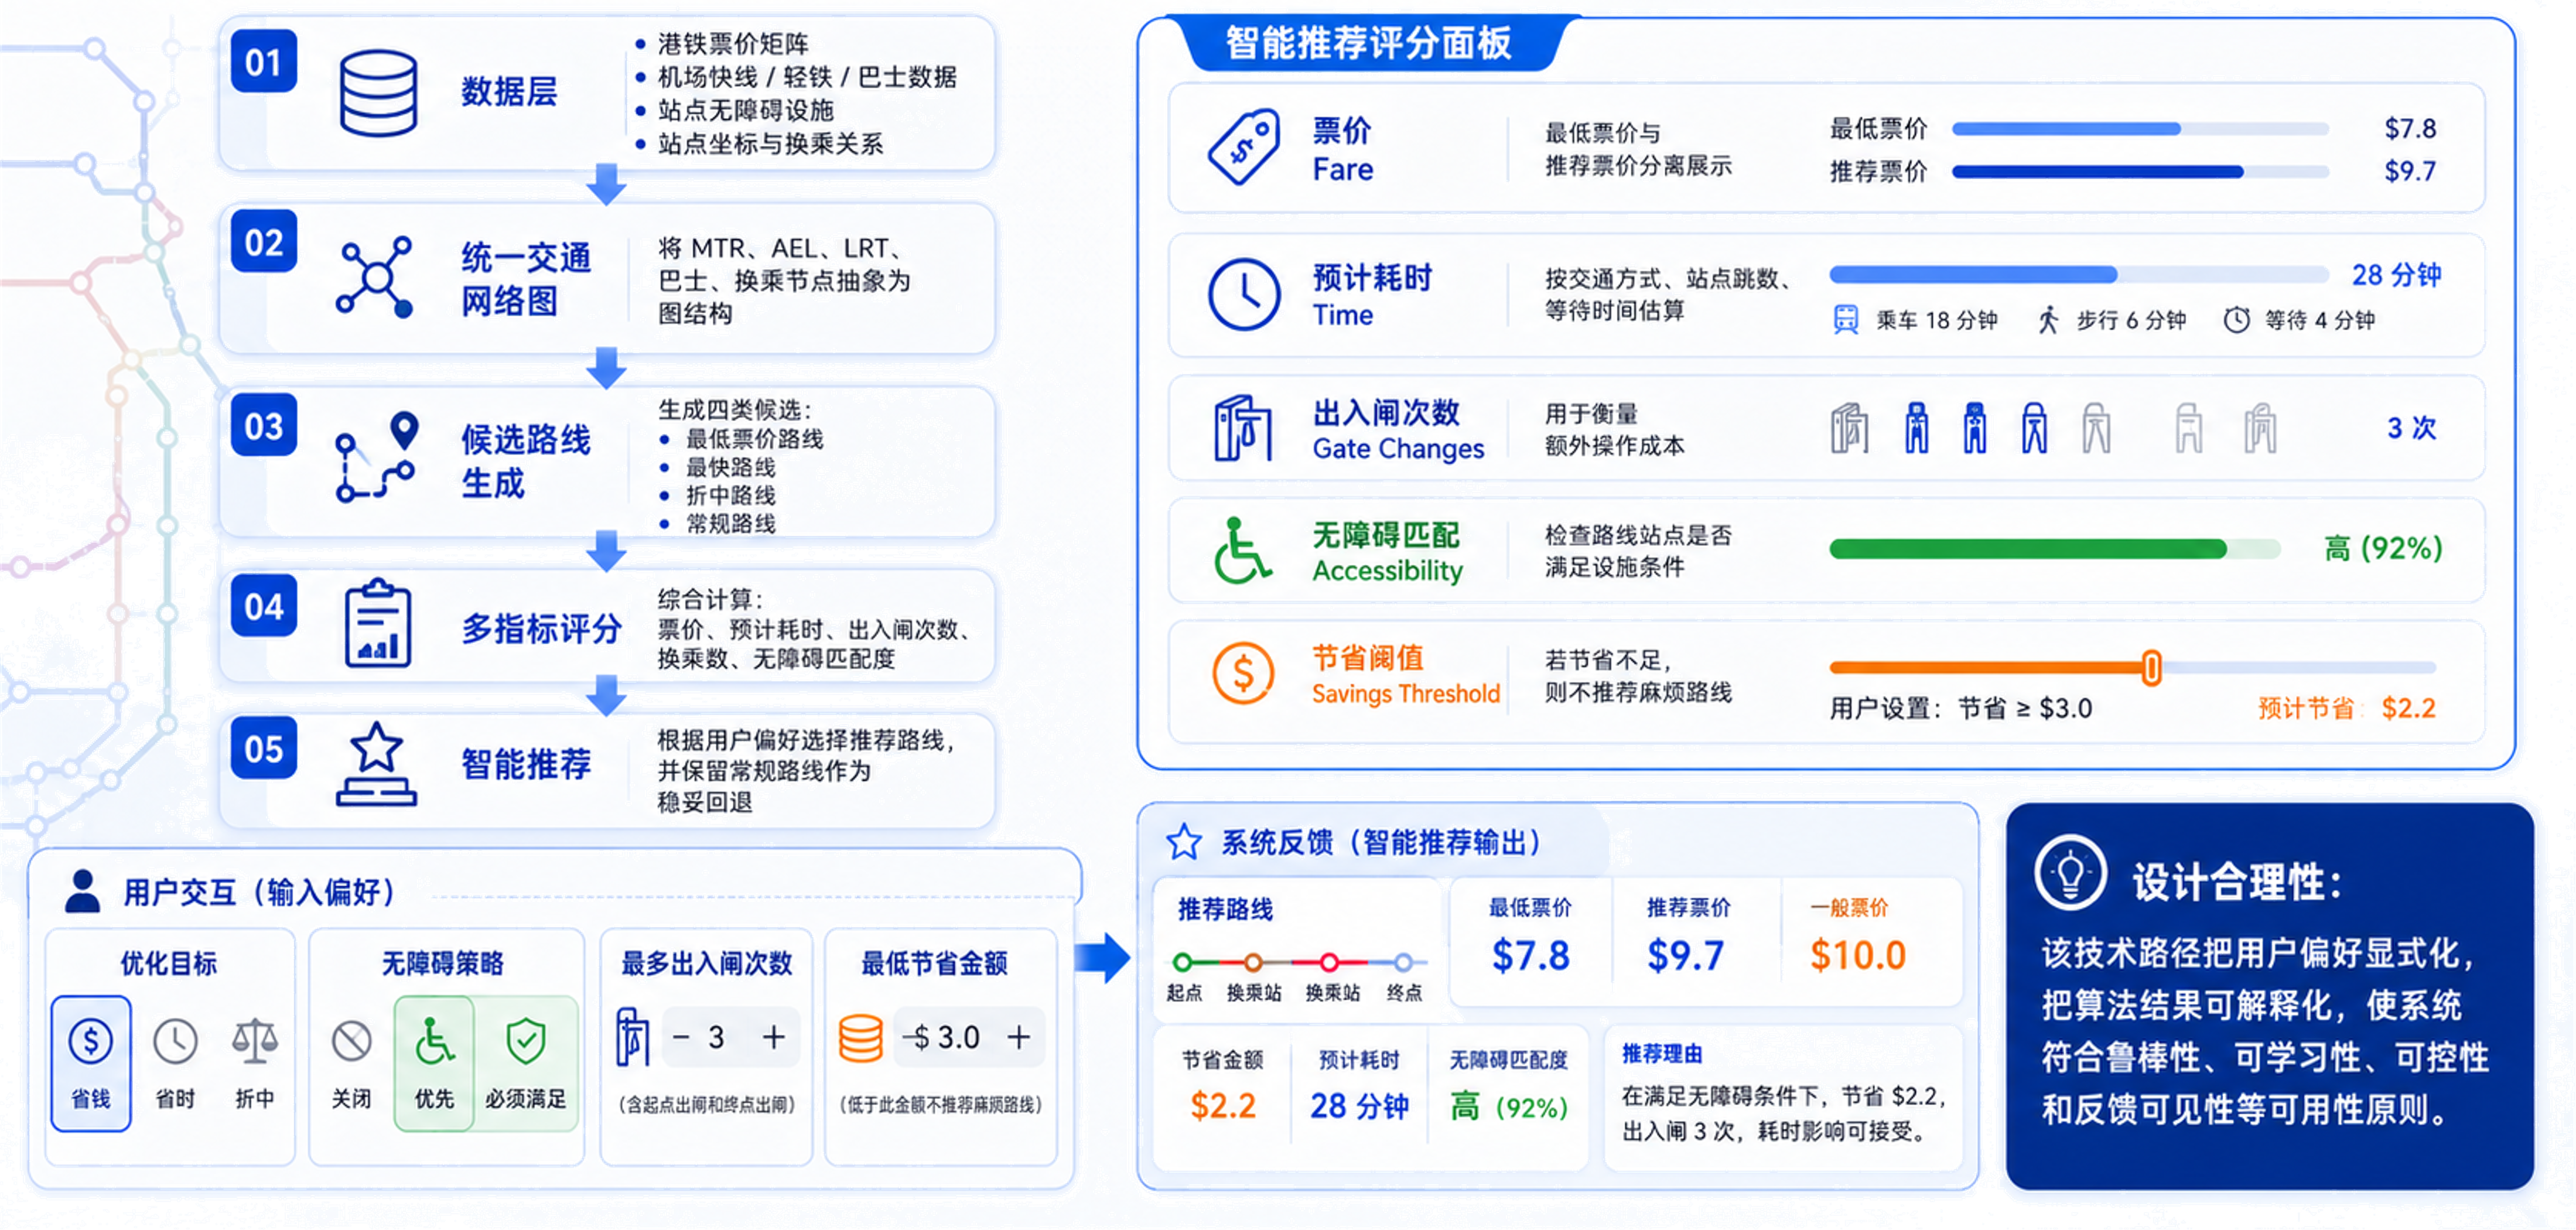
\includegraphics[width=0.95\textwidth,height=0.8\textheight,keepaspectratio]{Part 4-Page 3.png}
\end{frame}

% 第四页
\begin{frame}{项目可用性分析 —— 从“最低票价”到“可执行的交通决策”}
    \centering
    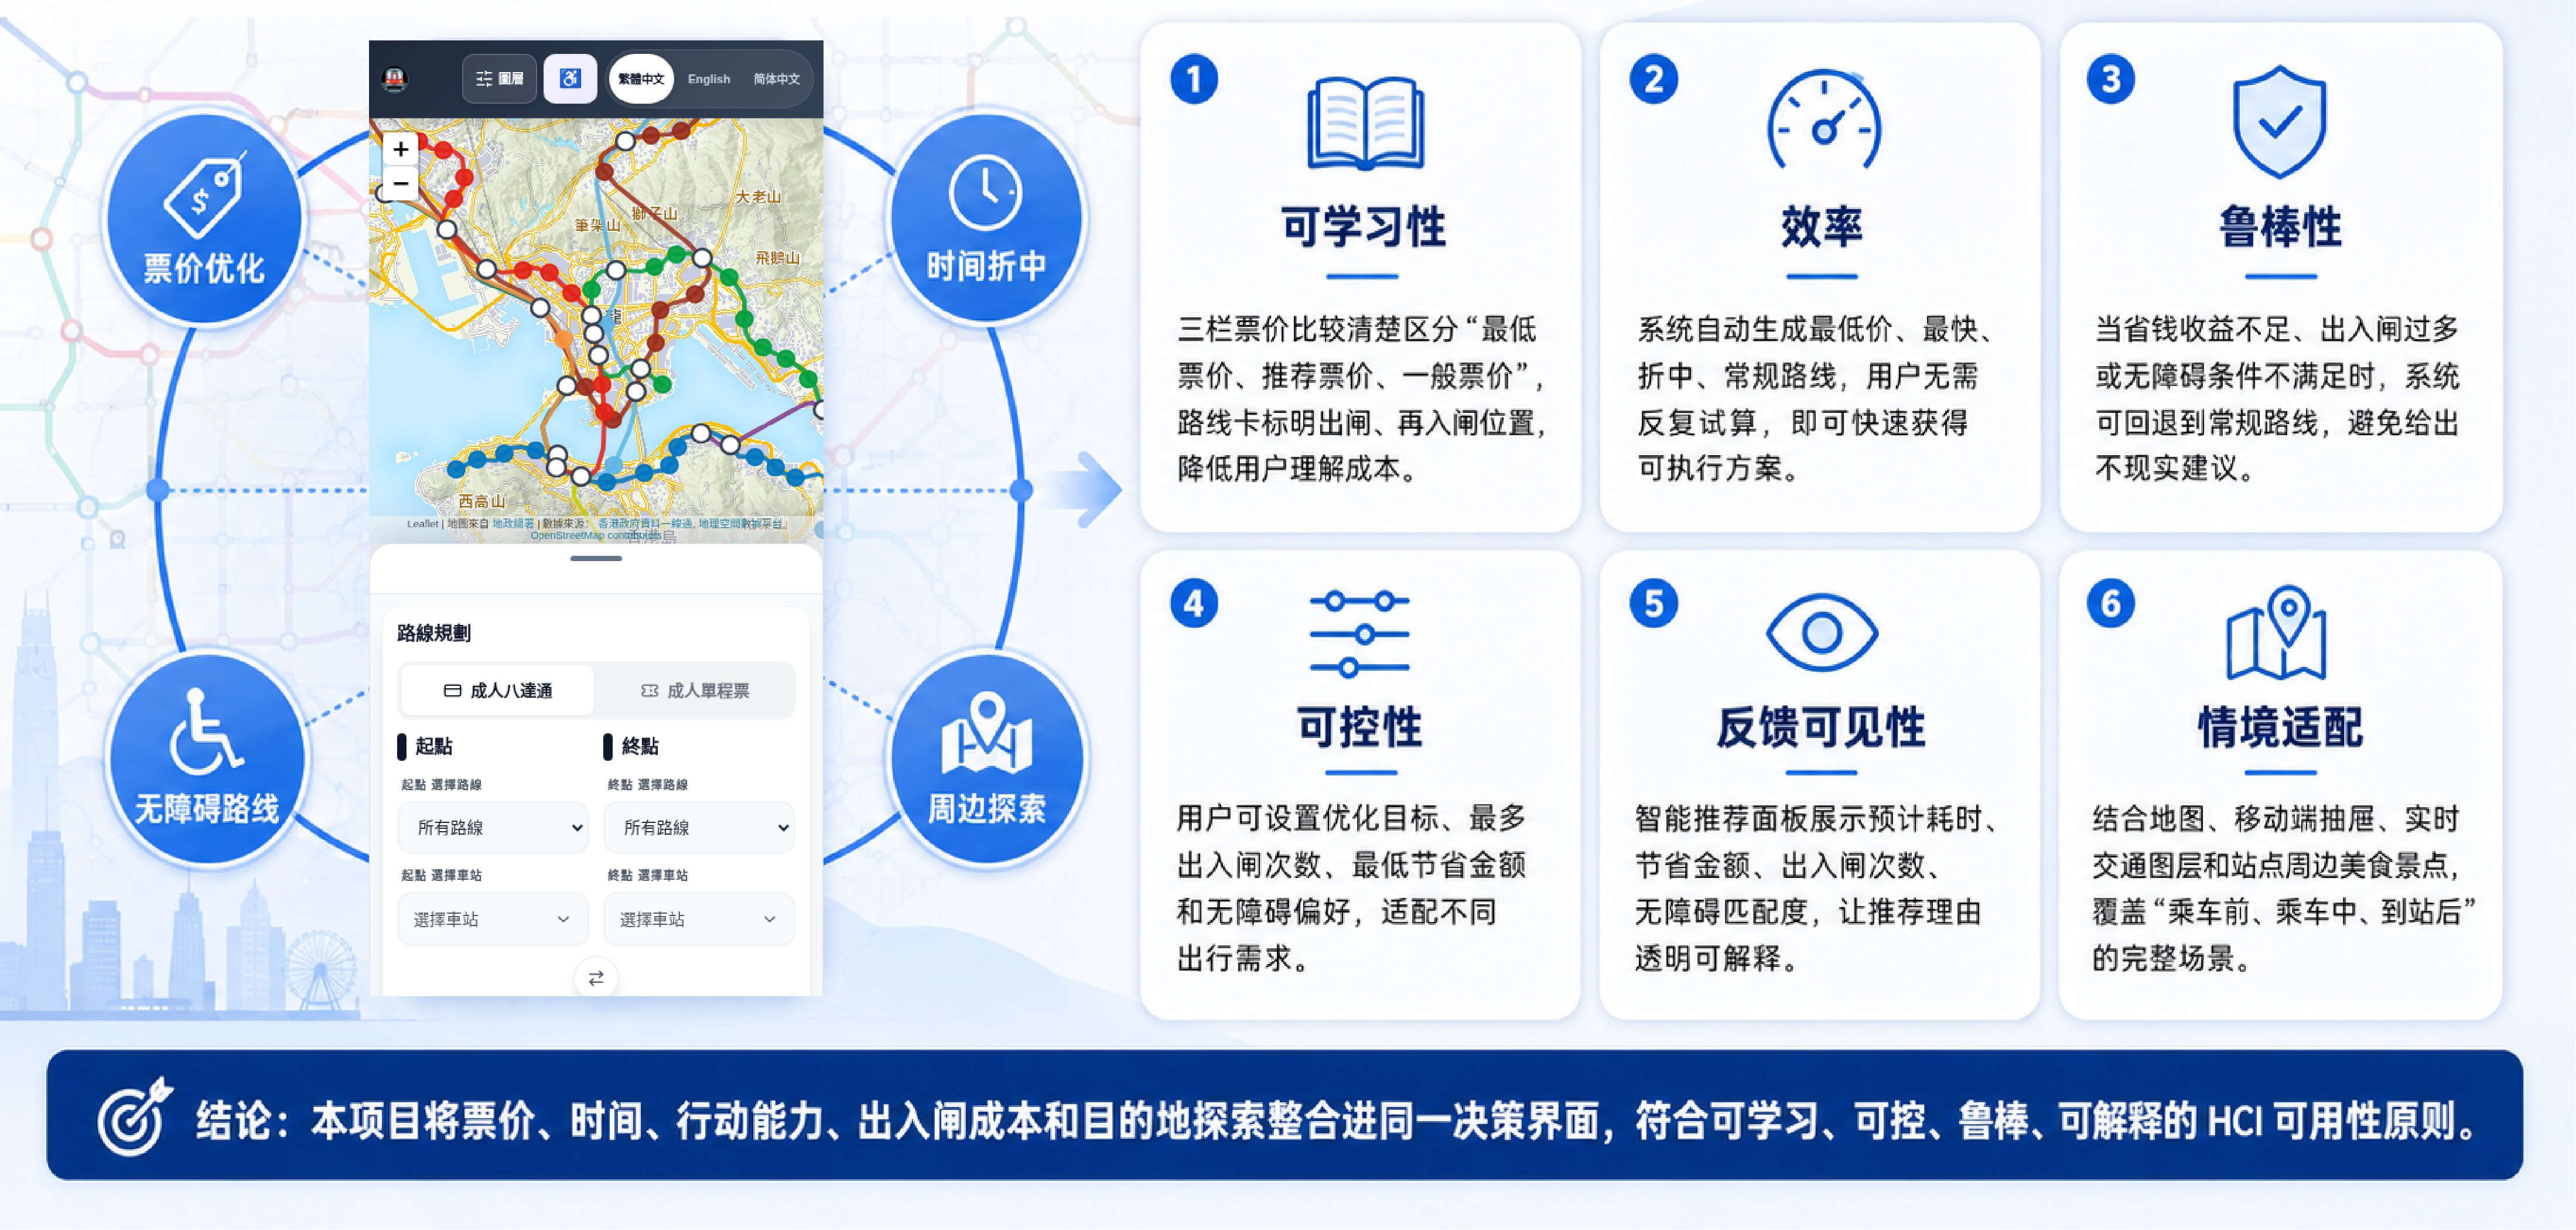
\includegraphics[width=0.95\textwidth,height=0.8\textheight,keepaspectratio]{Part 4-Page 4.png}
\end{frame}

% 第五页
\begin{frame}{竞品分析 —— 面向香港公共交通用户的票价智能优化与站点周边决策助手}
    \centering
    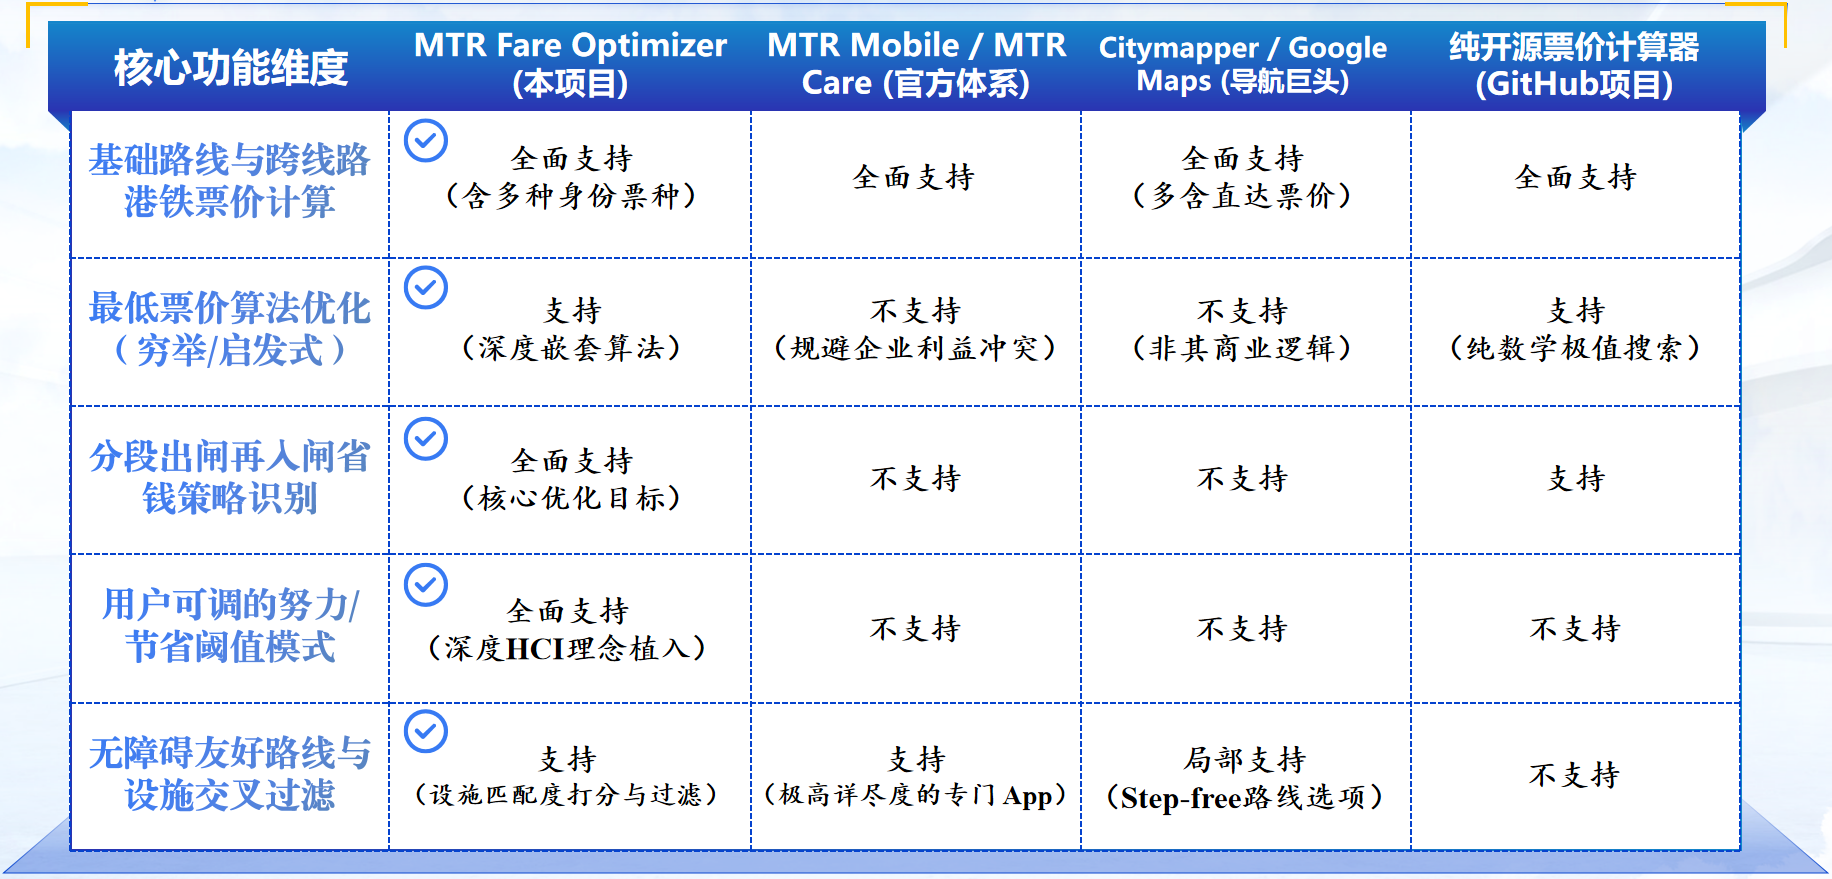
\includegraphics[width=0.95\textwidth,height=0.8\textheight,keepaspectratio]{Part 4-Page 5.png}
\end{frame}

% 第六页
\begin{frame}{竞品分析 —— 面向香港公共交通用户的票价智能优化与站点周边决策助手}
    \centering
    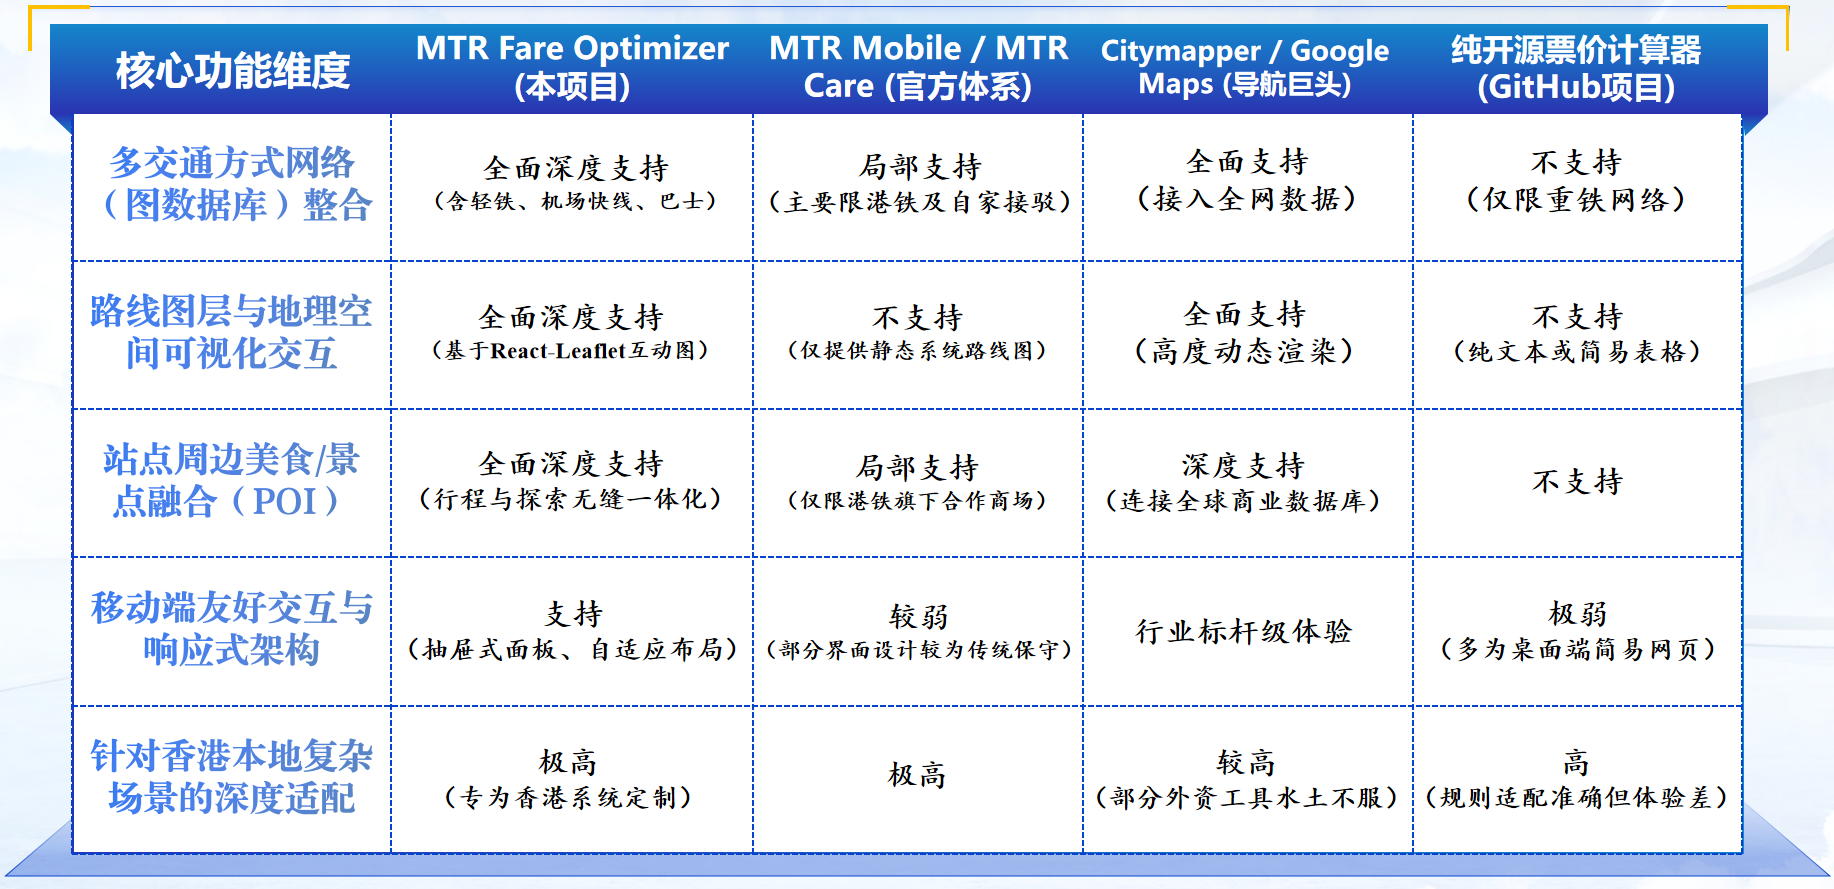
\includegraphics[width=0.95\textwidth,height=0.8\textheight,keepaspectratio]{Part 4-Page 6.png}
\end{frame}

% 第七页
\begin{frame}{用户体验调研 —— 检验项目在真实出行场景中的价值}
    \centering
    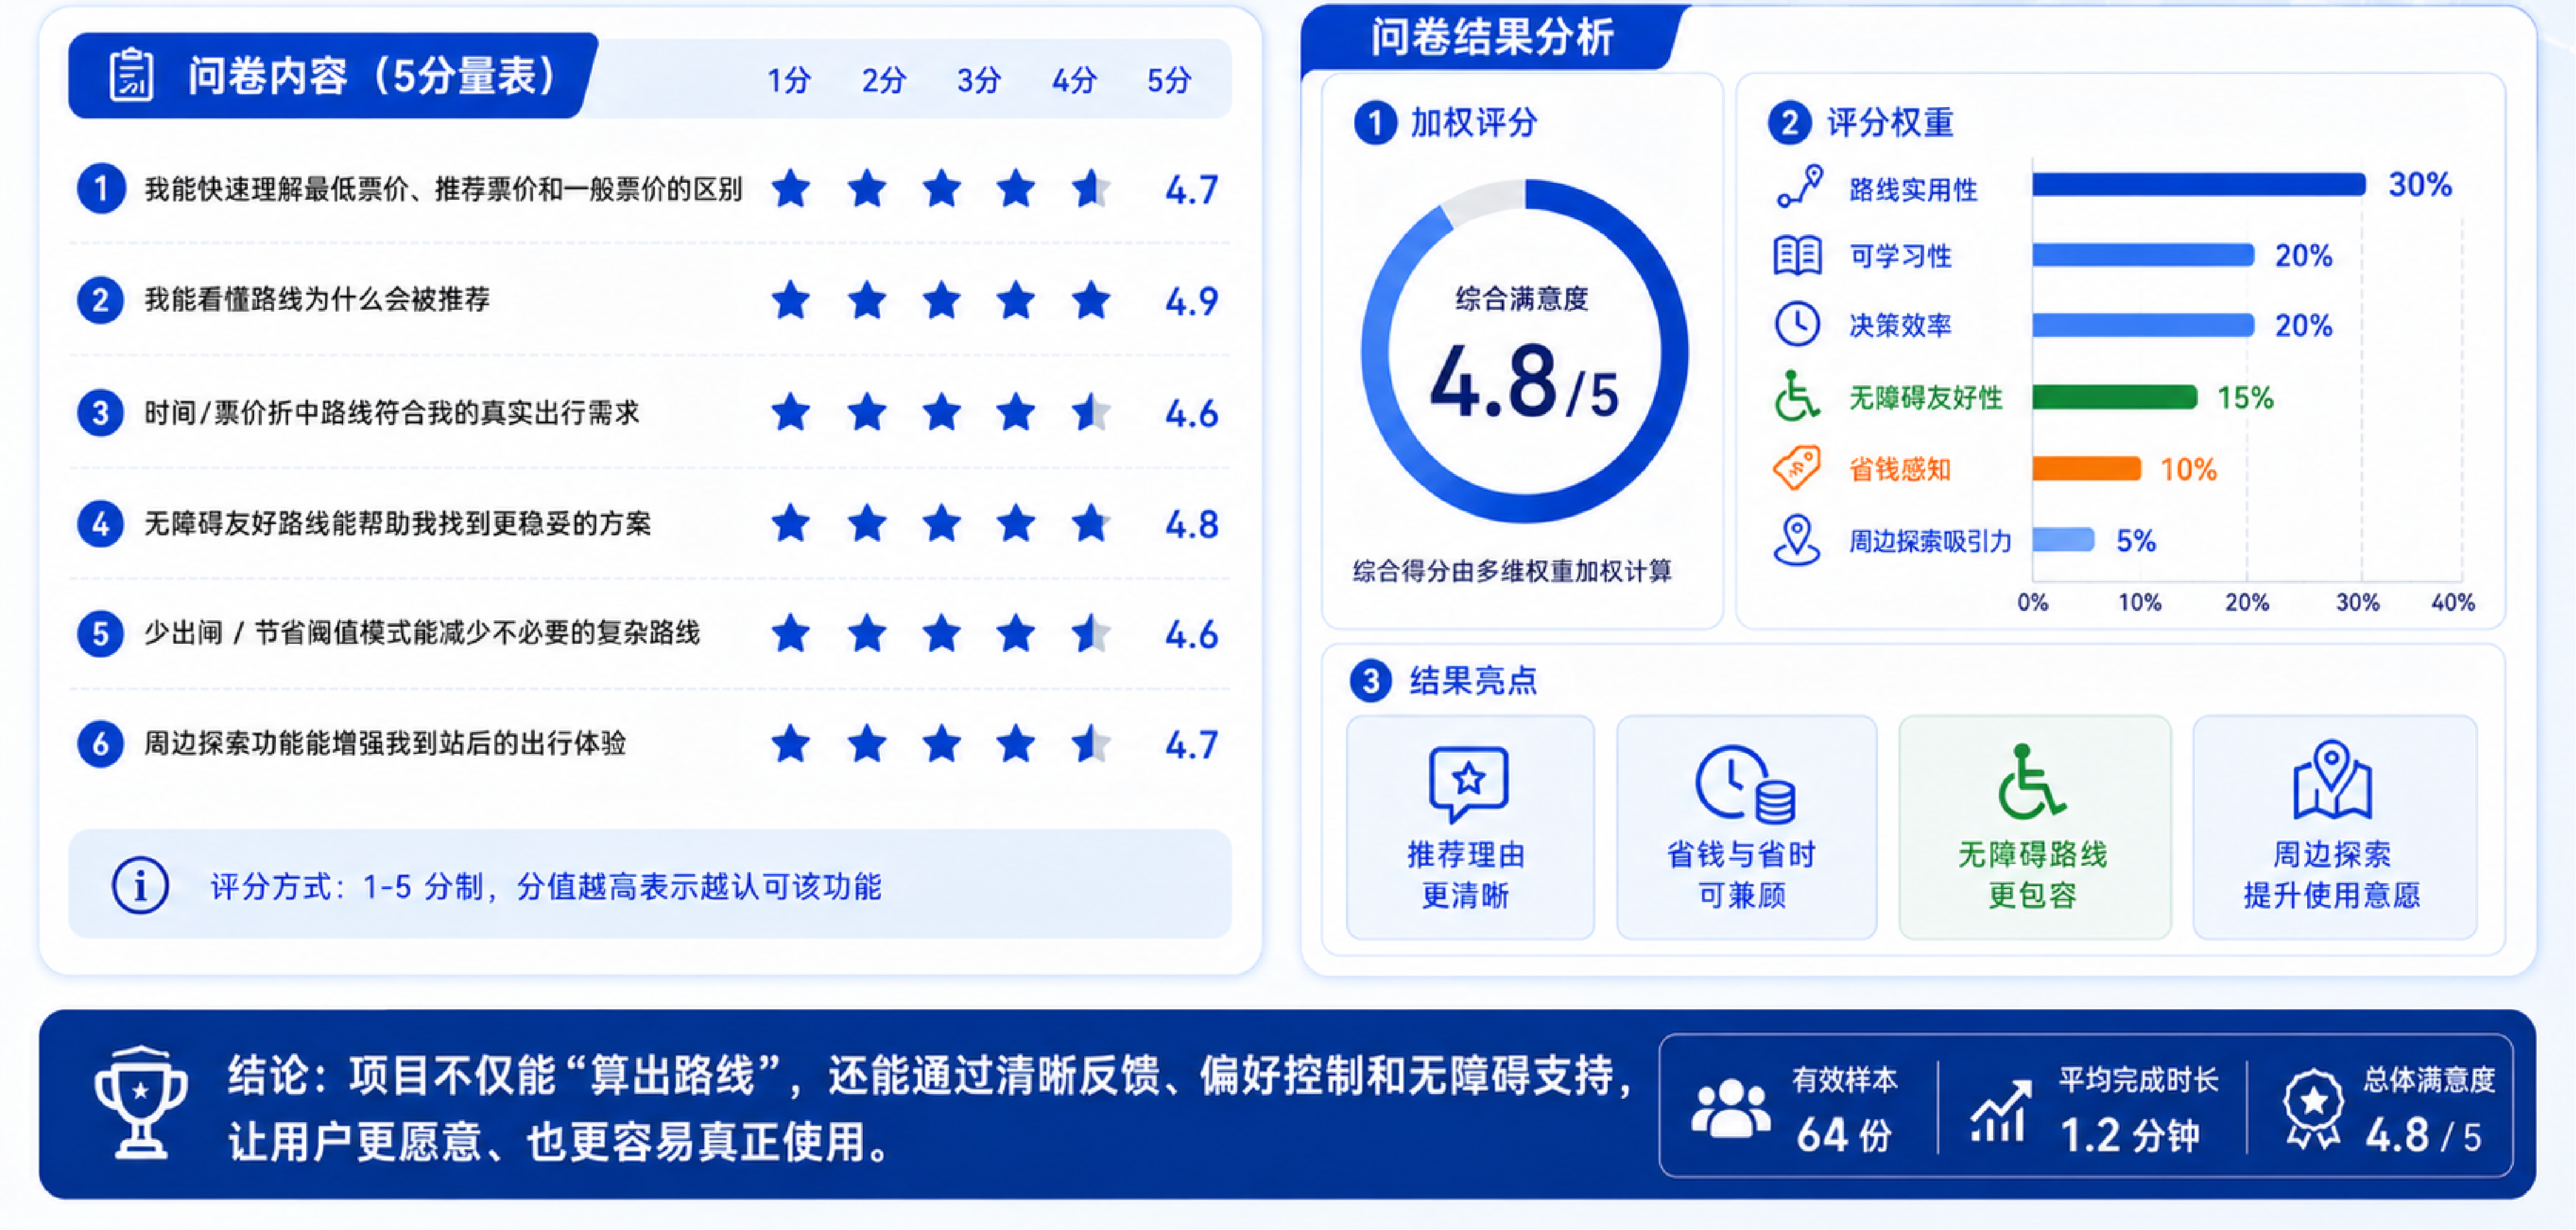
\includegraphics[width=0.95\textwidth,height=0.8\textheight,keepaspectratio]{Part 4-Page 7.png}
\end{frame}

\end{document}